% arara: clean: {
% arara: --> extensions:
% arara: --> ['log','aux','fdb_latexmk','fls','ilg','synctex.gz',
% arara: --> 'toc','out','bbl','bcf','blg','run.xml']
% arara: --> }
% arara: lualatex: { shell: yes }
% arara: biber
%! arara: lualatex: {
%! arara: --> shell: yes,
%! arara: --> synctex: yes,
%! arara: --> interaction: batchmode
%! arara: --> }
% arara: lualatex: { shell: true, interaction: nonstopmode }
% arara: clean: {
% arara: --> extensions:
% arara: --> ['log','aux','fdb_latexmk','fls','ilg','synctex.gz',
% arara: --> 'toc','out','bbl','bcf','blg','run.xml']
% arara: --> }
%=========================================================================================


\documentclass[
	11pt,
	a4paper,
	oneside
]{scrbook}

\usepackage[english, spanish,es-sloppy]{babel}
\selectlanguage{spanish}
\spanishdatedel

\usepackage{tasks}
\usepackage{ifluatex}
\ifluatex
	\usepackage{mathpazo}
	\usepackage{fontspec}
	\setmainfont{TeX Gyre Pagella}
\else
	\usepackage[T1]{fontenc}
	\usepackage{mathpazo}
\fi
\usepackage{pdfpages}
\usepackage{graphicx}
	\graphicspath{ {img} }

\usepackage{svg}
\usepackage{booktabs}
%\usepackage{longtable}
\usepackage{arydshln}
\usepackage{pdflscape}
\usepackage{wrapfig}
\usepackage{lipsum}

\usepackage{listings}
\usepackage{lstfiracode} % https://ctan.org/pkg/lstfiracode
%\lstset{
%	language=C++,
%	style=FiraCodeStyle,   % Use predefined FiraCodeStyle
%	basicstyle=\ttfamily,   % Use \ttfamily for source code listings
%	commentstyle=\color{orange},
%	moreliterate=
%	{;;}{{;;}}2
%	{///}{{///}}3
%}
\lstset{
	language=bash,
	style=FiraCodeStyle,
	basicstyle=\footnotesize\ttfamily,
	showstringspaces=false
}
\newcommand*\lstinputpath[1]{\lstset{inputpath=#1}}

\usepackage[
	backend = biber,
	style = numeric,
	defernumbers = true,
	sorting = ynt,
	maxbibnames = 4,
	maxcitenames = 4
]{biblatex}
\addbibresource{04_backmatter/references.bib}

\usepackage[
	pdfencoding=auto,
	colorlinks,
	citecolor=blue,
	linkcolor=red,
	pdfpagelabels
]{hyperref}% Hipervínculos


\renewcommand{\spanishchaptername}{Título}
\renewcommand{\spanishcontentsname}{Contenido}

\newcommand{\MVAt}{{\usefont{U}{mvs}{m}{n}\symbol{`@}}}
\newcommand{\flae}{\textbf{FLAE} }
\newcommand{\myCover}{
	
\includepdf{01_cover/Cover.pdf}
}
\newcommand{\myBackCover}{
	
\includepdf{01_cover/backcover.pdf}
}

\begin{document}
\hypersetup{pageanchor=false}
\frontmatter
	\myCover
	\setcounter{page}{0}
	% === Título de la portada ===
\begin{titlepage}
	\raggedleft 						% Alinear todo a la derecha
	\vspace*{\baselineskip}	% Espacios en blanco en la parte superior de la página
	
	{\Large
		Franz Victorio	\\
		Carlos Aznarán	\\
		Freider Achic		\\
		Renzo Q. Amao		\\
	}\vspace*{0.167\textheight}

	\bfseries{\LARGE Guía de inicio }\\[\baselineskip]
	
	{{\Huge Four Leaves}}\\[\baselineskip]
	
	\large Organización	\vfill	Evenhold

	\vspace{3\baselineskip} % La versión * solo va cuando no hay texto en la hoja donde se edita.
	
\end{titlepage}
	\chapter{Prefacio}

	\lipsum[1]
	\chapter{Prólogo}

	\lipsum[1]

	\hypersetup{pageanchor=true}
	\tableofcontents

\mainmatter
	\chapter{¿Qué es GNU/Linux?}

\lipsum[1]
\begin{wrapfigure}{l}{0.25\paperwidth}
	\centering
	\includesvg[width=0.24\paperwidth]{./img/gnu}
\end{wrapfigure}
\lipsum[1]

	\mintinline{latex}{article} and \mintinline{latex}{book} classes as well as to \mintinline{latex}{report} class. In \mintinline{latex}{article} class, however, the default position for the title information is at the top of the first text page rather than on a separate page. Also, it is not usual to request a table \mintinline{latex}{article} class.
\section{Subtítulo}

Los siguientes comandos de sección están disponibles:
\begin{quote}
 part \\
 chapter \\% \\ Fuerza una nueva linea
 section \\
 subsection \\
 subsubsection \\
 paragraph \\
 subparagraph
\end{quote}% Fin del texto indentado.

Pero tenga en cuenta que  a diferencia de las clases de \texttt{book} y \texttt{report}, la clase de \texttt{article} no tiene un comando \texttt{chapter}.

\chapter{Comandos básicos en GNU/Linux}

\lipsum[1]
\begin{wrapfigure}{r}{0.25\paperwidth}
	\centering
	
\includegraphics[width=0.24\paperwidth]{./img/linux/linux}
\end{wrapfigure}
\lipsum[1]

\begin{figure}[ht!]
	\centering
	
\includegraphics[width=0.2\paperwidth]{./img/bash}
	
\includegraphics[width=0.2\paperwidth]{./img/zshell}
	
\includegraphics[width=0.2\paperwidth]{./img/ohmyzsh}
\end{figure}


\section{Knowing your OS}
% TODO: uname, neofetch

\section{Escritorios}

\begin{figure}[ht!]
	\centering
	
\includegraphics[width=0.2\paperwidth]{./img/desktops/budgie}
	
\includegraphics[width=0.2\paperwidth]{./img/desktops/cinnamon}
	\includesvg[width=0.2\paperwidth]{./img/desktops/kde}
	
\includegraphics[width=0.2\paperwidth]{./img/desktops/gnome}
	\includesvg[width=0.2\paperwidth]{./img/desktops/plasma}
	
\includegraphics[width=0.2\paperwidth]{./img/desktops/lxde}
	
\includegraphics[width=0.2\paperwidth]{./img/desktops/lxqt}
	
\includegraphics[width=0.2\paperwidth]{./img/desktops/mate}
	
\includegraphics[width=0.2\paperwidth]{./img/desktops/xfce}
\end{figure}

\subsection{Distribuciones}

\begin{figure}[ht!]
	\centering
	\includesvg[width=0.2\paperwidth]{./img/linux/alpine}
	
\includegraphics[width=0.2\paperwidth]{./img/linux/android}
	
\includegraphics[width=0.2\paperwidth]{./img/linux/archlinux}
	
\includegraphics[width=0.2\paperwidth]{./img/linux/asteroidos}
	
\includegraphics[width=0.2\paperwidth]{./img/linux/centos}
	
\includegraphics[width=0.2\paperwidth]{./img/linux/chrome}
	\includesvg[width=0.2\paperwidth]{./img/linux/clearlinux}
	\includesvg[width=0.2\paperwidth]{./img/linux/debian}
	
\includegraphics[width=0.2\paperwidth]{./img/linux/kali}
	
\includegraphics[width=0.2\paperwidth]{./img/linux/kaos}
	
\includegraphics[width=0.2\paperwidth]{./img/linux/libreelec}
	
\includegraphics[width=0.2\paperwidth]{./img/linux/solus}
	
\includegraphics[width=0.2\paperwidth]{./img/linux/elementary}
	\includesvg[width=0.2\paperwidth]{./img/linux/uos}
	
\includegraphics[width=0.2\paperwidth]{./img/linux/ubuntu}
	\includesvg[width=0.2\paperwidth]{./img/linux/sailfish}
	\includesvg[width=0.2\paperwidth]{./img/linux/mx}
	
\includegraphics[width=0.2\paperwidth]{./img/linux/pisi}
	
\includegraphics[width=0.2\paperwidth]{./img/linux/mageia}
	\includesvg[width=0.2\paperwidth]{./img/linux/tails}
	
\includegraphics[width=0.2\paperwidth]{./img/linux/gentoo}
	
\includegraphics[width=0.2\paperwidth]{./img/linux/deepin}
	
\includegraphics[width=0.2\paperwidth]{./img/linux/fedora}
	
\includegraphics[width=0.2\paperwidth]{./img/linux/redhat}
	
\includegraphics[width=0.2\paperwidth]{./img/linux/raspbian}
	\includesvg[width=0.2\paperwidth]{./img/linux/opensuse}
	
\includegraphics[width=0.2\paperwidth]{./img/linux/manjaro}
\end{figure}

%\begin{landscape}
%\begin{table}[ht!]
%	\caption{Comparación de la línea de comando del gestión de software (fuente: \url{wiki.archlinux.org})}
%	\centering
%	\begin{tabular}{@{} p{110pt}:p{100pt}:l:p{102pt}:l @{}}
%		\toprule
%		Acción & Arch & Red Hat/Fedora & Debian/Ubuntu & SLES/openSUSE
%		\tabularnewline
%		\midrule
%		Instala un paquete por su nombre. & \lstinline|pacman -S| & \lstinline|dnf install| & \lstinline|apt install| & \lstinline|zypper install|
%		\tabularnewline
%		Elimina un paquete por su nombre. & \lstinline|pacman -Rs| & \lstinline|dnf remove| & \lstinline|apt remove| & \lstinline|zypper remove|
%		\tabularnewline
%		Busca un paquete por su nombre. & \lstinline|pacman -Ss| & \lstinline|dnf search| & \lstinline|apt search| & \lstinline|zypper search|
%		\tabularnewline
%		Actualiza los paquetes. & \lstinline|pacman -Syu| & \lstinline|dnf upgrade| & \lstinline|apt update &&|\newline \lstinline|apt upgrade| & \lstinline|zypper update|
%		\tabularnewline
%		Limpia la memoria\newline caché local. & \lstinline|pacman -Scc| & \lstinline|dnf clean all| & \lstinline|apt autoclean| & \lstinline|zypper clean|
%		\tabularnewline
%		Elimina dependencias innecesarias. & \lstinline|pacman -Rsn|\newline \lstinline|$(pacman -Qdtq)| & \lstinline|dnf autoremove| & \lstinline|apt autoremove| & \lstinline|zypper rm -u|
%		\tabularnewline
%		Muestra información\newline sobre un paquete. & \lstinline|pacman -Si| & \lstinline|dnf info| & \lstinline|apt show| & \lstinline|zypper info|
%		\tabularnewline
%		Lista de paquetes\newline instalados. & \lstinline|pacman -Q| & \lstinline|dnf list installed| & \lstinline|apt list --installed| & \lstinline|zypper search|\newline \lstinline|--installed-only|
%		\tabularnewline
%		Registra las acciones tomadas por el gestor de software. & \lstinline|/var/log/pacman.log| & \lstinline|dnf history| & \lstinline|/var/log/dpkg.log| & \lstinline|/var/log/zypp/history|
%		\tabularnewline
%		\bottomrule
%	\end{tabular}
%\end{table}
%\end{landscape}

%\begin{lstlisting}[style=cpp]
%// Hello.cpp
%#include <iostream>
%
%int main()
%{
%	std::cout << "Four leaves.\n";
%
%	return 0;
%}
%\end{lstlisting}
%
%\begin{lstlisting}[style=bash]
%#!/usr/bin/bash
%echo $SHELL
%\end{lstlisting}
	\chapter{Git + GitHub}

\section{Git}

\lipsum[1]
\begin{wrapfigure}{r}{0.25\paperwidth}
	
\includegraphics[width=0.24\paperwidth]{./img/git}
\end{wrapfigure}
\lipsum[1]

\begin{description}
	\item[Repositorio] Es una base de datos que contiene toda la información acerca de las versiones de los archivos en un proyecto, ubicado en una carpeta oculta \mintinline{console}{.git}.
	\item[Confirmación] Instantánea global de todos los archivos del proyecto con descripción de los cambios con respecto a la versión anterior.
	\item[Rama] Secuencia de commits que describe una rama (línea) de desarrollo. Un repositorio puede contener más de uno. La rama estándar se llama \mintinline{console}{master}.
	\item[Tag] Nombre persistente (identificador) para un commit, por ejemplo, cuando hace un lanzamiento público.
\end{description}

Antes de empezar a usar git, debemos tener instalado el sistema de control de versiones.

\begin{minted}{console}
four-leaves@me:~$ sudo apt update
four-leaves@me:~$ sudo apt install git-core
\end{minted}

Muy bien, ahora dos cosas deben ser configuradas:
\begin{minted}{console}
four-leaves@me:~$ git config --global user.name "testuser"
four-leaves@me:~$ git config --global user.email "testuser@example.com"
\end{minted}
%TODO: Nota: bashrc, bashprofile

Cree un repositorio git ingresando lo siguiente en el directorio superior del proyecto:
\begin{minted}{console}
four-leaves@me:~$ git init miProyecto
Initialized empty Git repository in ~/miProyecto.git/
\end{minted}
Esto ha creado un repositorio vacío, todavía no hay confirmaciones:
\begin{minted}{console}
four-leaves@me:~$ git status
On branch master

No commits yet

nothing to commit (create/copy files and use "git add" to track)
\end{minted}
% TODO: Explicar git remote
\begin{minted}{console}
.git
├── branches
├── config
├── description
├── HEAD
├── hooks
│   ├── applypatch-msg.sample
│   ├── commit-msg.sample
│   ├── fsmonitor-watchman.sample
│   ├── post-update.sample
│   ├── pre-applypatch.sample
│   ├── pre-commit.sample
│   ├── pre-merge-commit.sample
│   ├── prepare-commit-msg.sample
│   ├── pre-push.sample
│   ├── pre-rebase.sample
│   ├── pre-receive.sample
│   └── update.sample
├── info
│   └── exclude
├── objects
│   ├── info
│   └── pack
└── refs
├── heads
└── tags

9 directories, 16 files
\end{minted}

\subsection{Confirmaciones}
Una confirmación contiene
\begin{itemize}
	\item una instantánea de todos los archivos.
	\item la fecha de creación.
	\item el nombre y contenido con respecto al autor de los cambios.
	\item una lista de cambios.
	\item una lista de referencias a confirmaciones principales.
\end{itemize}
Las confirmaciones son identificadas usando un hash (suma de verificación) de su contenido, por ejemplo \mintinline{console}{5cd006a1c044b786ea8196636cd0b62e296dbbe5}.

Los hash de confirmación pueden abreviarse siempre que la abreviatura sea única.

Las confirmaciones no pueden cambiar: contenido diferente $\Rightarrow$ valor hash diferente.

\subsection{Ramas}

\begin{itemize}
	\item Una rama es una línea de desarrollo dentro de un repositorio.
	\item Los repositorios pueden contener un número arbitrario de ramas.
	\item \mintinline{console}{git status} puede decirle en qué rama se encuentra.
	\item Una rama siempre apunta a un \mintinline{console}{commit}.
	\item La creación de una nueva confirmación guarda la confirmación actual como principal y la rama luego apunta la nueva confirmación.
\end{itemize}

\subsection{Varios repositorios}

\begin{itemize}
	\item git puede sincronizar cambios entre repositorios.
	\item Los repositorios adicionales se llaman remotos.
	\item Las ramas de un repositorio remoto tienen el nombre del repositorio como prefijo.
	\item Puede clonar un repositorio remoto para obtener su contenido.
	\item No se pueden ver ramas de repositorios remotos directamente.
	\item En la primera revisión, git crea una rama de seguimiento.
	\item Los nuevos cambios se pueden descargar y combinar usando \mintinline{console}{git pull}.
\end{itemize}

\begin{table}[ht!]
	\caption{Comandos principales de alto nivel de git (fuente: \url{git-scm.com/docs})}
	\centering
	\begin{tabular}{@{} ll @{}}
	\toprule
	Comando & Breve descripción
	\tabularnewline
	\midrule
	\mintinline{console}{init} & Crea un repositorio de Git vacío o reinicialice uno existente.
	\tabularnewline
	\mintinline{console}{clone} & Clona un repositorio en un nuevo directorio.
	\tabularnewline
	\mintinline{console}{add} & Agrega contenido del archivo al índice.
	\tabularnewline
	\mintinline{console}{commit} & Registra los cambios en el repositorio.
	\tabularnewline
	\mintinline{console}{log} & Muestra registros de confirmación.
	\tabularnewline
	\mintinline{console}{diff} & Muestra cambios entre confirmaciones, confirmación y árbol de trabajo, etc.
	\tabularnewline
	\mintinline{console}{branch} & Enumera, crea o elimina ramas.
	\tabularnewline
	\mintinline{console}{checkout} & Cambia ramas o restaura archivos de árbol de trabajo.
	\tabularnewline
	\mintinline{console}{merge} & Une dos o más historias de desarrollo juntas.
	\tabularnewline
	\mintinline{console}{pull} & Obtenga e integre con otro repositorio o una sucursal local.
	\tabularnewline
	\mintinline{console}{push} & Actualiza las referencias remotas junto con los objetos asociados.
	\tabularnewline
	\bottomrule
	\end{tabular}
\end{table}

\section{GitHub}
\lipsum[1]
\begin{wrapfigure}{l}{0.15\paperwidth}
	
\includegraphics[width=0.14\paperwidth]{./img/github}
\end{wrapfigure}
\lipsum[1]

\section{GitLab}
\lipsum[1]
\begin{wrapfigure}{r}{0.15\paperwidth}
	\includesvg[width=0.14\paperwidth]{./img/gitlab}
\end{wrapfigure}
\lipsum[1]

\section{Automatización de compilación}

Organiza la construcción de su proyecto

Debe intentar ser eficiente y solo reconstruir lo que se requiere para mantener el ciclo corto de compilación-enlace-ejecución-depuración.

También puede intentar detectar propiedades del sistema de destino (a menudo el mismo que el host) y personalizar su programa en consecuencia.

También puede intentar proporcionar opciones de compilación para habilitar / deshabilitar opcionalmente las funciones de su proyecto.

También puede organizar pruebas de su proyecto.

Desea construir su proyecto lo más rápido posible.

Es posible que desee hacer que su proyecto sea portátil.

Escribir tu propio sistema de construcción es aburrido y tedioso.

Makefiles escritos a mano

Los desarrolladores de software especifican los objetivos y sus reglas de compilación.

Si escribió sus reglas correctamente, make asegura que solo se vuelvan a compilar los archivos de origen necesarios.

Perfecto para proyectos pequeños
\section{Lenguajes de marcado}

\subsection{Markdown}
\lipsum[1]
\begin{wrapfigure}{r}{0.2\paperwidth}
	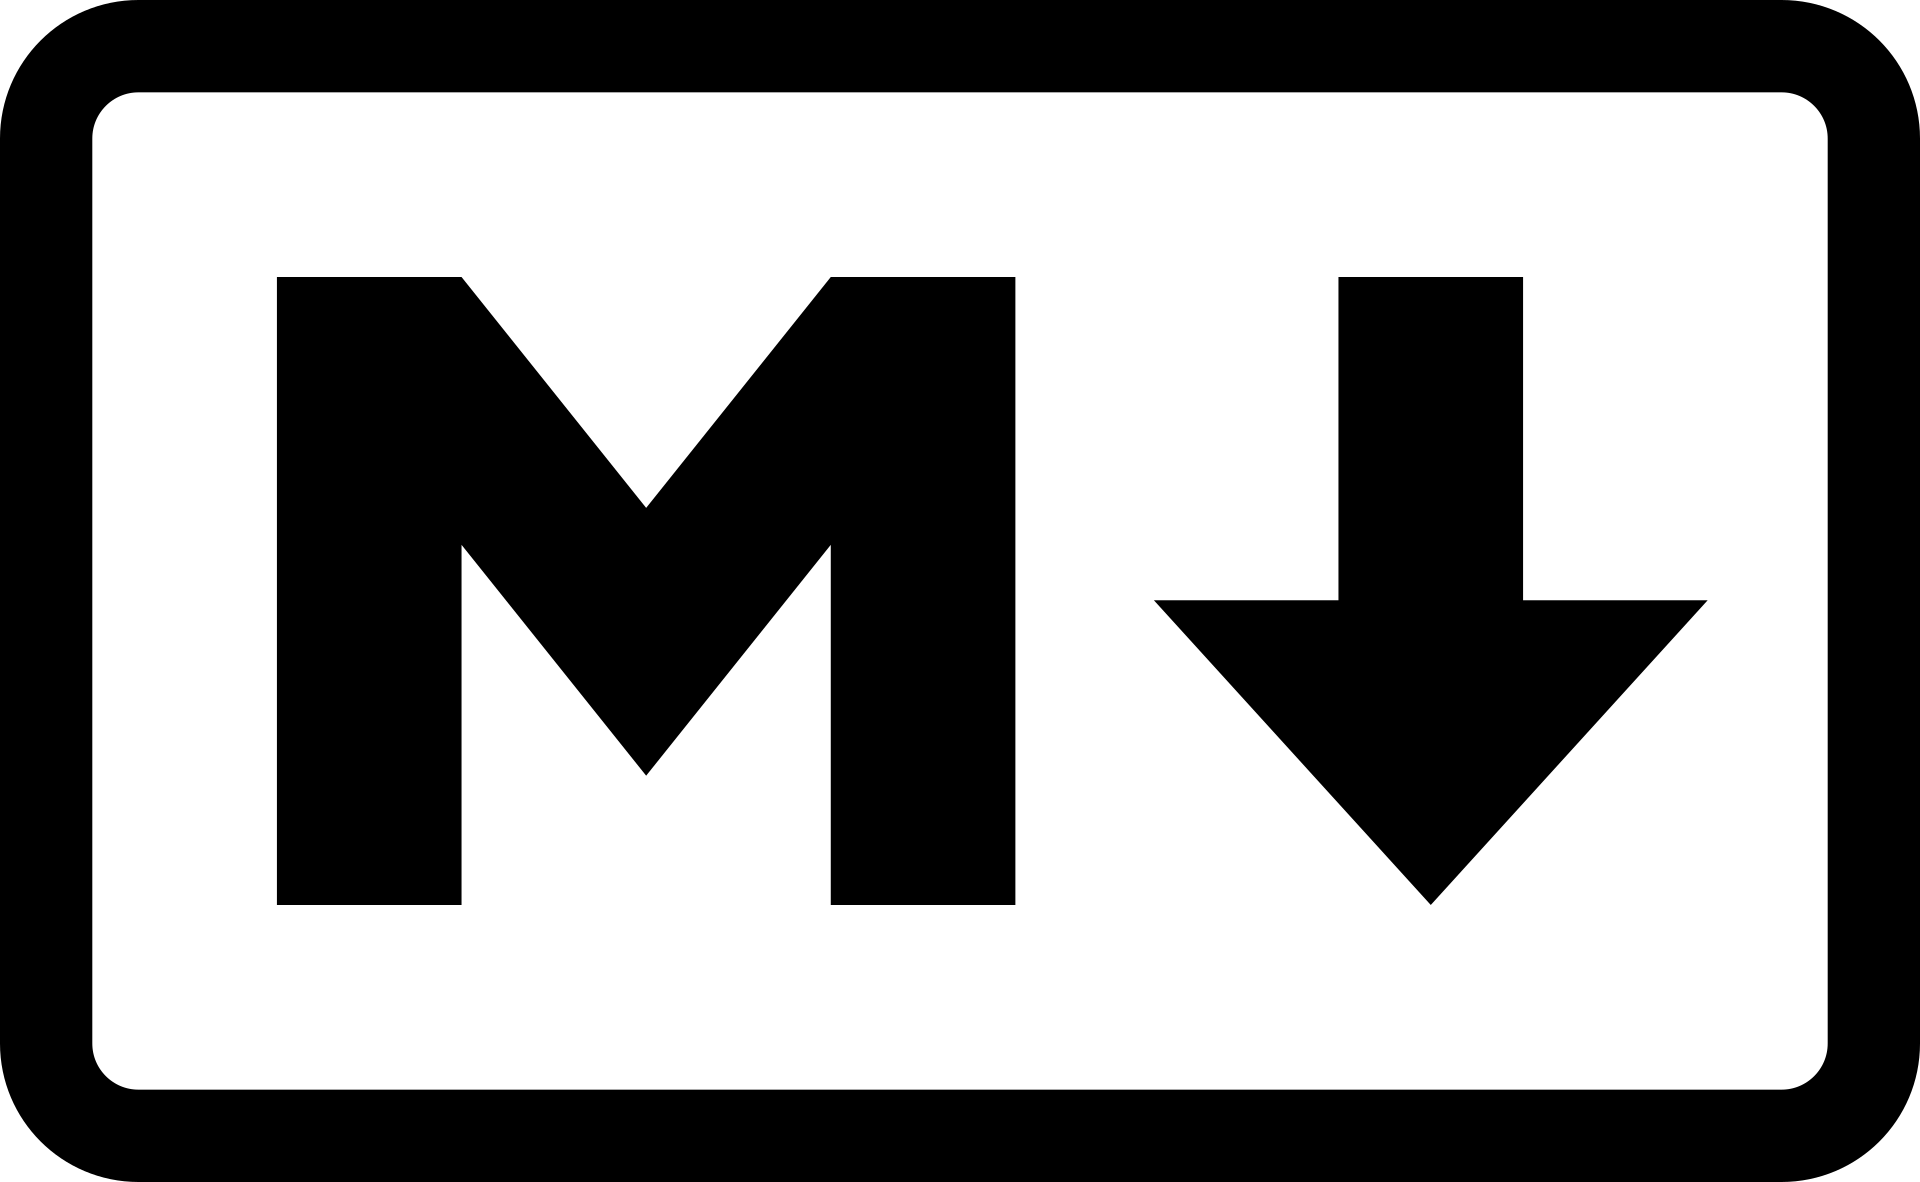
\includegraphics[width=0.19\paperwidth]{./img/markup/markdown}
\end{wrapfigure}
\lipsum[1]

\subsection{ReStructuredText}
\lipsum[1]
\begin{wrapfigure}{l}{0.2\paperwidth}
	
\includegraphics[width=0.19\paperwidth]{./img/markup/ReStructuredText}
\end{wrapfigure}
\lipsum[1]

\subsection{yaml}
\lipsum[1]
\begin{wrapfigure}{r}{0.2\paperwidth}
	
\includegraphics[width=0.19\paperwidth]{./img/markup/yaml}
\end{wrapfigure}
\lipsum[1]

\subsection{orgmode}
Vi and emacs are the most popular editors of UNIX and Linux worlds.

Their flexibility and size of functionalities ...
\lipsum[1]
\begin{wrapfigure}{l}{0.2\paperwidth}
	\includesvg[width=0.19\paperwidth]{./img/markup/orgmode}
\end{wrapfigure}
\lipsum[1]
	\chapter{Descripción de los editores de propósito general}

Nuestro trabajo es repetitivo por naturaleza. Cuando hacemos pequeños cambios en varias partes o moviéndonos alrededor entre regiones similares de un documento, repetimos varias acciones. Cualquier cosas que pueda seguir una línea repetitiva de flujo de trabajo nos ahorrará múltiple tiempo.

Vim está optimizado para la repetición. Su eficiencia proviene de la forma en que rastrea nuestras acciones más recientes. Podemos siempre repetir el último cambio con una sola pulsación de tecla. Por poderoso que parezca, es inútil a menos que aprendamos a diseñar nuestras acciones para que realicen una unidad de trabajo útil cuando se reproducen. Dominar este concepto es la clave para hacerse efectivo con Vim.

El comando punto es nuestro punto de partida. Este comando aparentemente simple es la más versátil herramienta en la caja, y entendiendo este es el primer paso hacia el dominio de Vim. Trabajaremos a través de un puñado de tareas de edición simples que se pueden ejecutar rápidamente completadas con el comando punto. Aunque cada tarea se ve bastante diferente de la siguiente, sus soluciones casi convergen. Identificaremos una fórmula de edición ideal, que requiere solo una pulsación de tecla para moverse y otra para ejecutar.

\begin{figure}[ht!]
\centering
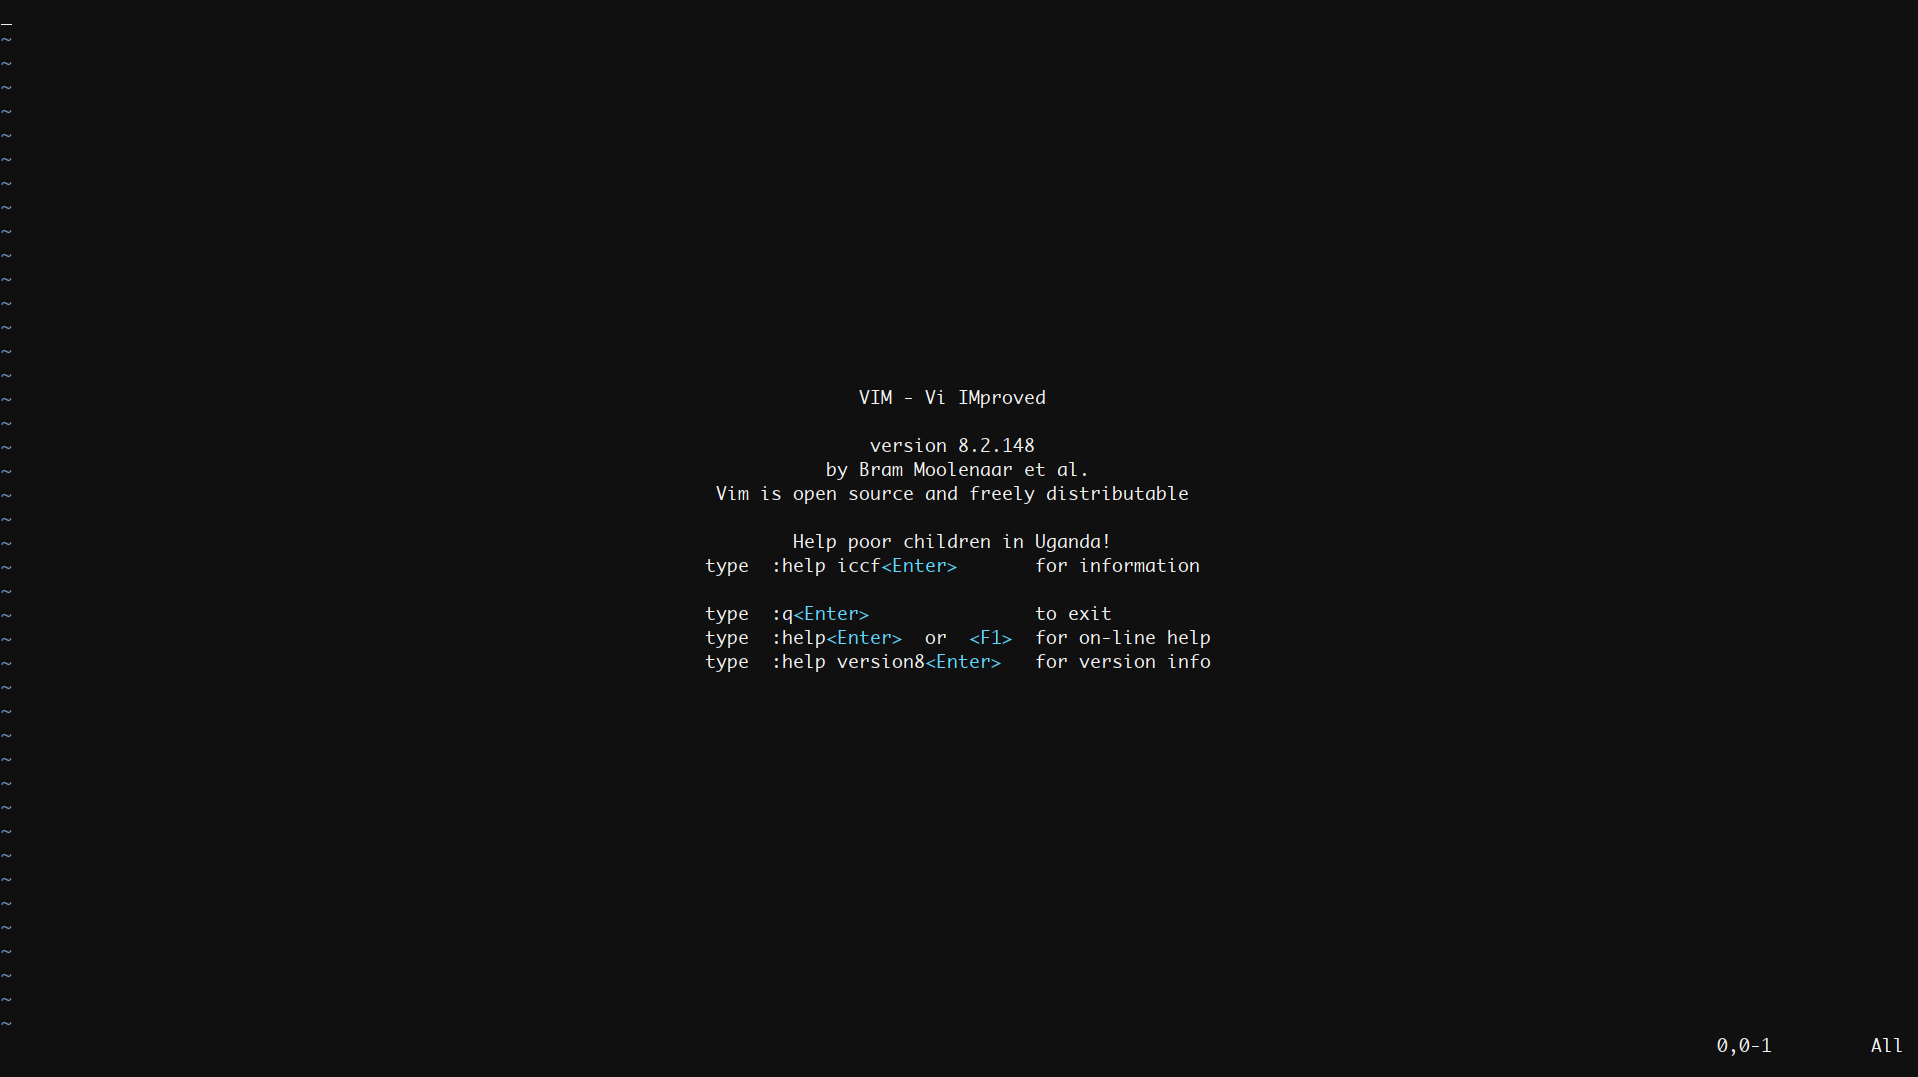
\includegraphics[width=0.8\paperwidth]{./img/VimStart}
\end{figure}

\begin{figure}[ht!]
	\centering
	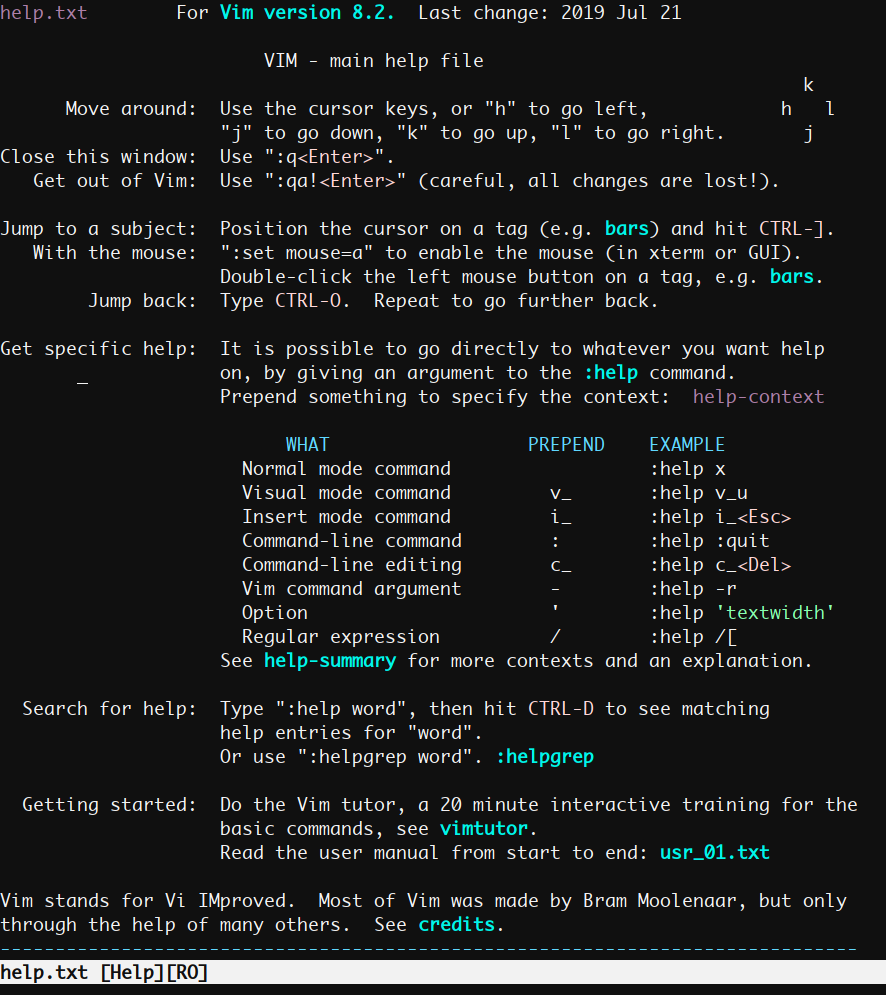
\includegraphics[width=0.8\paperwidth]{./img/VimHelp}
\end{figure}

\section{Vim}
Para entrar al modo de comandos debemos presionar
la tecla \keys{ESC} seguida del símbolo \keys{:}
(dos puntos), y para entrar al modo de edición tenemos que
presionar la tecla \keys{ESC} seguida de alguna de las
siguientes letras:

\mintinline{vim}{a:} entra en modo de edición y agrega el texto
tipeado justro detrás de la posición del cursor.

\mintinline{vim}{i:} entra en modo de edición e inserta el texto
justo delante de la posición actual del cursor.

\mintinline{vim}{A:} Añade el nuevo texto al final de la línea actual
indicada por el cursor.

\mintinline{vim}{I:} inserta el texto al comienzo de la línea indicada
por el cursor.

\mintinline{vim}{O:} inserta una nueva línea entre la línea inferior a la
posición del cursor.

* Para guardar el archivo y continuar editándolo entramos
al modo comando y tipeamos el comando \mintinline{vim}{:w}.

* Para guardar el archivo y salir del editor entramos al
modo comando y tipeamos el comando \mintinline{vim}{:wq}.

* Para salir del editor sin guardar el archivo, entramos al
modo comando y tipeamos el comando \mintinline{vim}{:q!}.

El próximo paso es aprendernos los comandos para desplazarnos
por el contenido de la ventana de Vi. Para todos los siguientes
atajos es necesario presionar antes la tecla ESC para entrar
en modo de comando:

\mintinline{vim}{w:} mover el cursor hacia la siguiente palabra.
\mintinline{vim}{e:} mover el cursor hacia el final de la palabra.
\mintinline{vim}{b:} mover el cursor hacia el comienzo de la palabra.
\mintinline{vim}{):} mover el cursor hacia el inicio de la próxima oración.
\mintinline{vim}{(:} mover el cursor hacia el inicio de la oración actual.
\mintinline{vim}|}:| mover el cursor hacia el inicio del próximo párrafo.
\mintinline{vim}|{:| mover el cursor hacia el inicio del párrafo actual.
\mintinline{vim}{G:} mover el cursor hacia el final del archivo.

También disponemos de algunas combinaciones de teclas para
desplazarnos por la ventana de edición:

\keys{\ctrl+F}: mueve una pantalla completa hacia adelante.
\keys{\ctrl+B}: mueve una pantalla completa hacia atrás.

Ahora vamos a aprender a modificar nuestro texto. El comando
más simple es r, que se encarga de reemplazar el carácter
actual por otro indicado justo a continuación del comando
(como por ejemplo rb). Para borrar caracteres disponemos del
comando x, que acepta prefijos numéricos para definir cuántos
caracteres se deben borrar (por ejemplo 10x). Por su parte. el
comando d es un poco más versátil. Vemos algunas combinaciones:

dw: borra desde la posición
(como por ejemplo)
\keys{\ctrl + F}

\lipsum[1]
\begin{wrapfigure}{r}{0.2\paperwidth}
	\includesvg[width=0.19\paperwidth]{./img/editors/vim}
\end{wrapfigure}
\lipsum[1]

\section{Emacs}

\lipsum[1]
\begin{wrapfigure}{l}{0.2\paperwidth}
	\includesvg[width=0.19\paperwidth]{./img/editors/emacs}
\end{wrapfigure}
\lipsum[1]

\section{Sublime}

\lipsum[1]
\begin{wrapfigure}{r}{0.2\paperwidth}
	\includesvg[width=0.19\paperwidth]{./img/editors/sublime}
\end{wrapfigure}
\lipsum[1]

\section{Visual Studio Code(ium)}

\lipsum[1]
\begin{wrapfigure}{l}{0.2\paperwidth}

\includegraphics[width=0.19\paperwidth]{./img/editors/vscodium}
\end{wrapfigure}
\lipsum[1]

\section{Atom}

\lipsum[1]
\begin{wrapfigure}{r}{0.2\paperwidth}
	
\includegraphics[width=0.19\paperwidth]{./img/editors/atom}
\end{wrapfigure}
\lipsum[1]

`manni' style on a white background:
\usemintedstyle{manni}
\begin{minted}{c}
char *test = "1000";
int *test_int = (int*) test;
printf("Machine is %s-endian", (test_int >> 1)? "big":"little");    
\end{minted}

`vim' style on a dark background:
\usemintedstyle{vim}
% note that minted seems to screw up the placment of the background here
\begin{minted}[bgcolor=black]{c}
char *test = "1000";
int *test_int = (int*) test;
printf("Machine is %s-endian", (test_int >> 1)? "big":"little");  
\end{minted}

Derived `myvim' style on a white background:
\usemintedstyle{myvim}
\begin{minted}{c}
char *test = "1000";
int *test_int = (int*) test;
printf("Machine is %s-endian", (test_int >> 1)? "big":"little");  
\end{minted}
	\chapter{\LaTeX}

\lipsum[1]
\begin{wrapfigure}{r}{0.2\paperwidth}
	\includesvg[width=0.19\paperwidth]{./img/latex}
\end{wrapfigure}
\lipsum[1]

\section{arara}

\lipsum[1]
\begin{wrapfigure}{l}{0.2\paperwidth}
	
\includegraphics[width=0.19\paperwidth]{./img/arara}
\end{wrapfigure}
\lipsum[1]
	\chapter{Introducción al desarrollo web}

\section{HTML}

\lipsum[1]
\begin{wrapfigure}{r}{0.2\paperwidth}
	
\includegraphics[width=0.19\paperwidth]{./img/html}
\end{wrapfigure}
\lipsum[1]

\section{CSS}

\lipsum[1]
\begin{wrapfigure}{l}{0.2\paperwidth}
	
\includegraphics[width=0.19\paperwidth]{./img/css}
\end{wrapfigure}
\lipsum[1]

\section{Javascript}

\lipsum[1]
\begin{wrapfigure}{r}{0.2\paperwidth}
	
\includegraphics[width=0.19\paperwidth]{./img/javascript}
\end{wrapfigure}
\lipsum[1]
	\chapter{Preprocesadores}

\section{pug (HTML)}

\lipsum[1]
\begin{wrapfigure}{r}{0.2\paperwidth}
	\includesvg[width=0.19\paperwidth]{./img/pug}
\end{wrapfigure}
\lipsum[1]

\section{stylus (CSS)}

\lipsum[1]
\begin{wrapfigure}{r}{0.2\paperwidth}
	\includesvg[width=0.19\paperwidth]{./img/stylus}
\end{wrapfigure}
\lipsum[1]
	\chapter{Node.JS}

\lipsum[1]
\begin{wrapfigure}{r}{0.2\paperwidth}
	
\includegraphics[width=0.19\paperwidth]{./img/node}
\end{wrapfigure}
\lipsum[1]
	\chapter{Backend}

\section{Express.JS}

\lipsum[1]
\begin{wrapfigure}{r}{0.2\paperwidth}
	
\includegraphics[width=0.19\paperwidth]{./img/express}
\end{wrapfigure}
\lipsum[1]

\section{MongoDB}

\lipsum[1]
\begin{wrapfigure}{r}{0.2\paperwidth}
	
\includegraphics[width=0.19\paperwidth]{./img/mongodb}
\end{wrapfigure}
\lipsum[1]
	\chapter{Algoritmos}

\lipsum[1]
\begin{wrapfigure}{r}{0.2\paperwidth}
	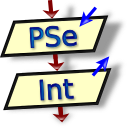
\includegraphics[width=0.19\paperwidth]{./img/pseint}
\end{wrapfigure}
\lipsum[1]

\backmatter
	\nocite{*}
\printbibliography[title={Bibliografía},heading=bibintoc]
	\myBackCover

\end{document}